\documentclass{article}

% Language setting
% Replace `english' with e.g. `spanish' to change the document language
\usepackage[english]{babel}

% Set page size and margins
% Replace `letterpaper' with`a4paper' for UK/EU standard size
\usepackage[letterpaper,top=2cm,bottom=2cm,left=3cm,right=3cm,marginparwidth=1.75cm]{geometry}

% Useful packages
\usepackage{amsmath}
\usepackage{amssymb}
\usepackage{graphicx}
\usepackage{enumitem}
\usepackage[colorlinks=true, allcolors=blue]{hyperref}

\usepackage{hyperref}
\hypersetup{
    colorlinks=true,
    linkcolor=blue,
    filecolor=magenta,      
    urlcolor=cyan,
    pdftitle={Math 185 Homework 3},
    pdfpagemode=FullScreen,
    }

\urlstyle{same}

\usepackage{tikz-cd}

%%%%%%%%%%% Box pacakges and definitions %%%%%%%%%%%%%%
\usepackage[most]{tcolorbox}
\usepackage{xcolor}

% Define the colors
\definecolor{boxheader}{RGB}{0, 51, 102}  % Dark blue
\definecolor{boxfill}{RGB}{173, 216, 230}  % Light blue

% Define the tcolorbox environment
\newtcolorbox{mathdefinitionbox}[2][]{%
    colback=boxfill,   % Background color
    colframe=boxheader, % Border color
    fonttitle=\bfseries, % Bold title
    coltitle=white,     % Title text color
    title={#2},         % Title text
    enhanced,           % Enable advanced features
    attach boxed title to top left={yshift=-\tcboxedtitleheight/2}, % Center title
    boxrule=0.5mm,      % Border width
    sharp corners,      % Sharp corners for the box
    #1                  % Additional options
}
%%%%%%%%%%%%%%%%%%%%%%%%%

\usepackage{biblatex}
\addbibresource{sample.bib}


%%%%%%%%%%% New Commands %%%%%%%%%%%%%%
\newcommand*{\T}{\mathcal T}
\newcommand*{\cl}{\text cl}


\newcommand{\ket}[1]{|#1 \rangle}
\newcommand{\bra}[1]{\langle #1|}
\newcommand{\inner}[2]{\langle #1 | #2 \rangle}
\newcommand{\R}{\mathbb{R}}
\newcommand{\C}{\mathbb{C}}
\newcommand{\V}{\mathbb{V}}
\newcommand{\Hilbert}{\mathcal{H}}
\newcommand{\oper}{\hat{\Omega}}
\newcommand{\lam}{\hat{\Lambda}}

\newcommand{\bigslant}[2]{{\raisebox{.2em}{$#1$}\left/\raisebox{-.2em}{$#2$}\right.}}
\newcommand{\restr}[2]{{% we make the whole thing an ordinary symbol
  \left.\kern-\nulldelimiterspace % automatically resize the bar with \right
  #1 % the function
  \vphantom{\big|} % pretend it's a little taller at normal size
  \right|_{#2} % this is the delimiter
  }}
%%%%%%%%%%%%%%%%%%%%%%%%%%%%%%%%%%%%%%%


\newtcolorbox{dottedbox}[1][]{%
    colback=white,    % Background color
    colframe=white,    % Border color (to be overridden by dashrule)
    sharp corners,     % Sharp corners for the box
    boxrule=0pt,       % No actual border, as it will be drawn with dashrule
    boxsep=5pt,        % Padding inside the box
    enhanced,          % Enable advanced features
    overlay={\draw[dashed, thin, black, dash pattern=on \pgflinewidth off \pgflinewidth, line cap=rect] (frame.south west) rectangle (frame.north east);}, % Dotted line
    #1                 % Additional options
}

\tcbset{theostyle/.style={
    enhanced,
    sharp corners,
    attach boxed title to top left={
      xshift=-1mm,
      yshift=-4mm,
      yshifttext=-1mm
    },
    top=1.5ex,
    colback=white,
    colframe=blue!75!black,
    fonttitle=\bfseries,
    boxed title style={
      sharp corners,
    size=small,
    colback=blue!75!black,
    colframe=blue!75!black,
  } 
}}

\newtcbtheorem[number within=section]{Theorem}{Theorem}{%
  theostyle
}{thm}

\newtcbtheorem[number within=section]{Definition}{Definition}{%
  theostyle
}{def}



\title{Math H185 Homework 3}
\author{Keshav Balwant Deoskar}

\begin{document}
\maketitle


%%%%%%%%%%%%%%%%%%%%%%%%%%%%%%%%%%%%%%%%%%%%%%%%%%%%%%%%%%%%%%%%%
\begin{mathdefinitionbox}{Question 1}
\vskip 0.5cm
Let $r > 0$. For each $n \in \mathbb{Z}$, calculate 
\[ \int_{\partial B_r(0)} \overline{z}^n  dz \]
\end{mathdefinitionbox}
%%%%%%%%%%%%%%%%%%%%%%%%%%%%%%%%%%%%%%%%%%%%%%%%%%%%%%%%%%%%%%%%%

\vskip 0.5cm
\underline{\textbf{Proof:}}

\vskip 0.5cm
\begin{align*}
  \int_{\partial B_r(0)} \overline{z}^n dz &= \int_{\partial B_r(0)} \overline{z}^n \frac{z^n}{z^n} dz \\
  &= \int_{\partial B_r(0)} \frac{\left(|z|^2\right)^n}{z^n} dz 
\end{align*}

\vskip 0.5cm
But on $\partial B_r(0)$, we have $|z| = r$, so 

\begin{align*}
  \ int_{\partial B_r(0)} \overline{z}^n dz  &= r^{2n} \int_{\partial B_r(0)} \frac{1}{z^n} dz \\
\end{align*}

And, from lecture, we know that 
\begin{dottedbox}
  \begin{align*}
    \int_{\partial B_r(0)} z^m dz &= \begin{cases}
      0, m \neq -1 \\
      2\pi i, m = -1
    \end{cases} \\
    \implies \int_{\partial B_r(0)} \frac{1}{z^n} dz &= \begin{cases}
      0,  n\neq 1 \\
      2\pi i, n = 1
    \end{cases} 
  \end{align*}
\end{dottedbox}

\vskip 0.5cm
Thus, we have 
\begin{align*}
\boxed{  \int_{\partial B_r(0)} \overline{z}^n dz = \begin{cases}
  0, \;\;\;\;n \neq 1 \\
  r^{2n} \cdot 2\pi i, n = 1
\end{cases}}
\end{align*}

\vskip 0.5cm
\hrule 
\vskip 0.5cm




%%%%%%%%%%%%%%%%%%%%%%%%%%%%%%%%%%%%%%%%%%%%%%%%%%%%%%%%%%%%%%%%%
\begin{mathdefinitionbox}{Question 2}
\vskip 0.5cm
Show that if $f : \C \setminus \{0\}  \rightarrow \C$ is holomorphic on all of $\C \setminus \{0\}$, then
\[ \int_{\partial B_r(0)} f(z)dz \]
is independent of $r$.
\end{mathdefinitionbox}
%%%%%%%%%%%%%%%%%%%%%%%%%%%%%%%%%%%%%%%%%%%%%%%%%%%%%%%%%%%%%%%%%

\vskip 0.5cm
\underline{\textbf{Proof:}}

For any $r, r' > 0$ such that $r' < r$, let $U$ be the annulus formed by the circles of radii $r, r'$ around the origin. Then, the boundary $\partial U$ is $\partial B_r(0) \cup \partial B_{r'}(0)^{-}$ where the $(-)$ superscript is meant to denote the reverse orientation.

\begin{center}
  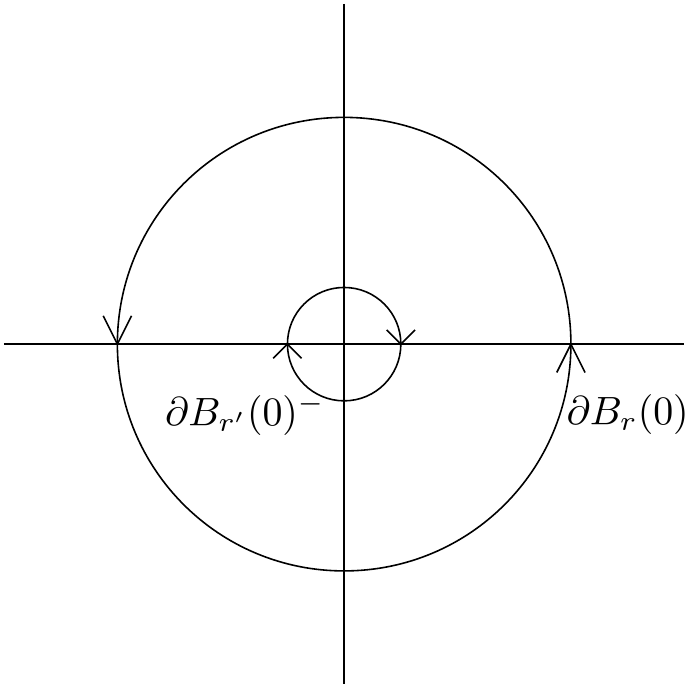
\includegraphics[scale=0.35]{Q2.png}
\end{center}

We know from Cauchy's Theorem that if $f : \Omega \subseteq_{open} \rightarrow \C$ is holomorphic on $\Omega$ and $\gamma$ is some path in $\Omega$, then 
\[ \int_{\gamma} f(z) dz = 0 \]

So, the integral we're interested in calculating is 
\begin{align*}
  0 &= \int_{\partial U} f(z) dz \\
  &= \int_{\partial B_r(0) \;\cup\; \partial B_{r'}(0)^{-}} f(z) dz \\
  &= \int_{\partial B_r(0)} f(z) dz + \int_{\partial B_{r'}(0)^{-}} f(z) dz \\
  &= \int_{\partial B_r(0)} f(z) dz - \int_{\partial B_{r'}(0)} f(z) dz
\end{align*}

\[ \implies \boxed{\int_{\partial B_r(0)} f(z) dz = \int_{\partial B_{r'}(0)} f(z) dz} \]

\vskip 0.25cm
This shows that the integral is independent of the radius of $r$ of the ball around the origin, given that $f$ is holomorphic on $\C \setminus \{0\}$.

\vskip 0.5cm
\hrule 
\vskip 0.5cm


%%%%%%%%%%%%%%%%%%%%%%%%%%%%%%%%%%%%%%%%%%%%%%%%%%%%%%%%%%%%%%%%
\begin{mathdefinitionbox}{Question 3}
\vskip 0.5cm
Let $f(z) = 3z^3 + z^2 + 4z + 1$. Calculate 
\[ \int_{\partial B_r(0)} f(z)z^n dz \]
for $r > 0$ and every $n \in \mathbb{Z}$.
\end{mathdefinitionbox}
%%%%%%%%%%%%%%%%%%%%%%%%%%%%%%%%%%%%%%%%%%%%%%%%%%%%%%%%%%%%%%%%%

\vskip 0.5cm
\underline{\textbf{Solution:}}

We already know that 
\[ \int_{\partial B_r(0)} z^m = \begin{cases}
  0, m \neq -1 \\
  2\pi i, m = -1
\end{cases} \]

\vskip 0.5cm
The $n \geq 0$ case is simple as the functions $f(z)$ and $z^n$ are both holomorphic at all points $z_0 \in \C$, so their product is also holomorphic at all points in $\C$. Then, Cauchy's Theorem tells us 
\[ \int_{\partial B_r(0)} f(z)z^n dz = 0 \] 


\vskip 0.5cm
For $n \leq -1$, it helps to break into cases. The integral we're trying to evaluate is
\begin{align*}
  \int_{\partial B_r(0)} f(z)z^n dz &= \int_{\partial B_r(0)} 3z^3 \cdot z^n dz + \int_{\partial B_r(0)} z^2 \cdot z^n dz + \int_{\partial B_r(0)} 4z \cdot z^n dz + \int_{\partial B_r(0)} 1 \cdot z^n dz \\
  &= 3\int_{\partial B_r(0)}z^{n+3} dz + \int_{\partial B_r(0)} z^{n+2} dz + 4\int_{\partial B_r(0)} z^{n+1} dz + \int_{\partial B_r(0)} z^n dz 
\end{align*}

\vskip 0.5cm
So, let's consider the following:

\begin{enumerate}[label=(\alph*)]
  \item \underline{$n = -1$:} In this case, the last integral survives while the others vanish, so 
  \[ \int_{\partial B_r(0)} f(z) z^n dz =  \int_{\partial B_r(0)} f(z) z^{-1} dz = 2\pi i \]

  \item \underline{$n = -2$:} In this case, the $z^{n+1}$ integral survives whereas the other vanish, so
  \[ \int_{\partial B_r(0)} f(z) z^n dz = 4 \cdot \int_{\partial B_r(0)} f(z) z^{-1} dz = 4 \cdot (2\pi i) \]

  \item \underline{$n = -3$:} In this case, the $z^{n+2}$ integral survives whereas the other vanish, so
  \[ \int_{\partial B_r(0)} f(z) z^n dz =  \int_{\partial B_r(0)} f(z) z^{-1} dz = 2\pi i \]

  \item \underline{$n = -4$:} In this case, the $z^{n+3}$ integral survives whereas the other vanish, so
  \[ \int_{\partial B_r(0)} f(z) z^n dz = 3 \cdot \int_{\partial B_r(0)} f(z) z^{-1} dz = 3 \cdot (2\pi i) \]

  \item \underline{$n \leq -5$:} In this case, all of the exponents are less than or equal to $(-2)$. So, all of the integrals are separately equal to zero, making the total integral vanish.
\end{enumerate}

In conclusion, 
\[ \boxed{ \int_{\partial B_r(0)} f(z) z^n dz = \begin{cases}
  0, n \geq 0 \text{ or } n \leq -5 \\
  2\pi i, n = -1 \\
  8\pi i, n = -2 \\
  2\pi i, n = -3 \\
  6\pi i, n = -4 \\
\end{cases} } \]

\vskip 0.5cm
\hrule 
\vskip 0.5cm




%%%%%%%%%%%%%%%%%%%%%%%%%%%%%%%%%%%%%%%%%%%%%%%%%%%%%%%%%%%%%%%%
\begin{mathdefinitionbox}{Question 4}
\vskip 0.5cm
Calculate 
\[ I = \int_{\partial B_r(0)} \frac{e^{\sin(\cos(z))}}{z - \frac{\pi}{2}} dz \]
for $r = 1$, $r = 2$.
\end{mathdefinitionbox}
%%%%%%%%%%%%%%%%%%%%%%%%%%%%%%%%%%%%%%%%%%%%%%%%%%%%%%%%%%%%%%%%%

\vskip 0.5cm
\underline{\textbf{Solution:}}

\vsize 0.5cm
\begin{enumerate}[label=(\alph*)]
  \item \underline{$r = 1$:} We notice that the integrand has a pole at $z = \pi/2 \approx 1.57 > 1$, so there exist no poles of the function in $B_1(0)$. The integrand is holomorphic in $B_1(0)$, so by Cauchy's Theorem, the integral evaluates to zero.
  
  \[ \boxed{I = 0} \]


  \vskip 0.5cm
  \item Cauchy's Formula tells us that if $f : \Omega \subseteq_{open} \C \rightarrow \C$ is holomorphic on $\Omega$ (or in fact, even just on $\Omega \setminus \{z_0\}$) then 
  \[ f(w) = \frac{1}{2\pi i} \int_{\partial B_r(z_0)} \frac{f(w)}{w - z_0} dw \]

  So, 
  \begin{align*}
    \int_{\partial B_2(0)} \frac{e^{\sin(\cos(z))}}{\left(z - \frac{\pi}{2}\right)} dz &= 2\pi i \cdot ^{\sin(\cos(\pi / 2))} = 2\pi i \cdot  e^{sin(1)}
  \end{align*}

  \[ \boxed{I = 2\pi i e^{\sin(1)}} \]
\end{enumerate}


\vskip 0.5cm
\hrule 
\vskip 0.5cm


%%%%%%%%%%%%%%%%%%%%%%%%%%%%%%%%%%%%%%%%%%%%%%%%%%%%%%%%%%%%%%%%%
\begin{mathdefinitionbox}{Question 5}
\vskip 0.5cm
Suppose that $f(z)$ is analytic on a domain containing $\overline{B_r(z)}$. Using Cauchy's formulas, prove that 
\[ f(z) = \frac{1}{2\pi} \int_{0}^{2\pi} f(z + re^{i\theta}) d\theta \]

This is called the \emph{Mean Value Property}. More generally, prove also that 
\[ f^{(n)}(z) = \frac{n!}{2\pi r^n} \int_0^{2\pi} f(z + re^{i\theta}) e^{-in\theta} d\theta \]
\end{mathdefinitionbox}
%%%%%%%%%%%%%%%%%%%%%%%%%%%%%%%%%%%%%%%%%%%%%%%%%%%%%%%%%%%%%%%%%

\vskip 0.5cm
\underline{\textbf{Proof:}}

Since we have a function $f(z)$ which is analytic on a domain containing $\overline{\mathbb{B}_r(z)}$, we can apply Cauchy's formula to find that 
\[ f(z) = \frac{1}{2\pi i} \int_{\partial B_r(z)} \frac{f(w)}{w - z} dw \]

Now, the $r-$ball can be parametrized as $\gamma(\theta) = z + re^{i\theta}$ for $\theta \in [0, 2\pi]$. So, 
\begin{align*}
  f(z) &= \frac{1}{2\pi i} \int_{\partial B_r(z)} \frac{f(w)}{w - z} dw \\
  &=\frac{1}{2\pi i} \int_{0}^{2 \pi} \frac{f(z + re^{i\theta})}{(z + re^{i\theta}) - z} \times \left( ie^{i\theta} \right) d\theta \\
  &=\frac{1}{2\pi i} \int_{0}^{2 \pi} \frac{f(z + re^{i\theta})}{+ re^{i\theta}} \times \left( ie^{i\theta} \right) d\theta \\
  &=\frac{1}{2\pi i} \int_{0}^{2 \pi}f(z + re^{i\theta})  d\theta 
\end{align*}

This gives us the Mean Value Property. More generally, we know from Cauchy's Integral formula that 

\[ f^{(n)}(z) = \frac{n!}{2\pi i } \int_{\partial B_r(z)} \frac{f(w)}{(w-z)^{n+1}} dw \]  

So, once again, parametrizing the ball using $\gamma(\theta) = z + re^{i\theta}$ where $\theta \in [0, 2\pi]$ we have 
\begin{align*}
  f^{(n)}(z) &= \frac{n!}{2\pi i } \int_{\partial B_r(z)} \frac{f(w)}{(w-z)^{n+1}} dw \\
  &= \frac{n!}{2\pi i } \int_{0}^{2\pi} \frac{f(z + re^{i\theta})}{(z + re^{i\theta}-z)^{n+1}} \cdot  \left( i re^{i\theta} \right)d\theta \\
  &= \frac{n!}{2\pi i } \int_{0}^{2\pi} \frac{f(z + re^{i\theta})}{(re^{i\theta})^{n+1}} \cdot  \left( i re^{i\theta} \right)d\theta \\
  &= \frac{n!}{2\pi} \int_{0}^{2\pi} f(z + re^{i\theta}) \frac{\left(re^{i\theta} \right)}{(re^{i\theta})^{n+1}} d\theta \\
  &= \frac{n!}{2\pi r^n} \int_{0}^{2\pi} f(z + re^{i \theta }) \cdot e^{-i n \theta} d\theta \\
\end{align*}
as desired.
\vskip 0.5cm
\hrule 
\vskip 0.5cm





%%%%%%%%%%%%%%%%%%%%%%%%%%%%%%%%%%%%%%%%%%%%%%%%%%%%%%%%%%%%%%%%%
\begin{mathdefinitionbox}{Question 6}
\vskip 0.5cm
Calculate 
\[ \int_{\partial B_5(0)}\frac{\overline{z}}{z-1} dz\]

Warning: Recall that $\overline{z}$ is not holomorphic, so Cauchy's formula does not directly apply to it. Nevertheless, a clever trick will save the day.
\end{mathdefinitionbox}
%%%%%%%%%%%%%%%%%%%%%%%%%%%%%%%%%%%%%%%%%%%%%%%%%%%%%%%%%%%%%%%%%

\vskip 0.5cm
\underline{\textbf{Solution:}}

\vskip 0.5cm
Note that, although $\overline{z}$ is not holomorphic anywhere -- making the entire integrand not holomorphic anywhere -- we can multiple the numerator and denominator with $z$ to get:

\begin{align*}
  \int_{\partial B_5(0)} \frac{\overline{z}z}{z(z-1)}dz &= \int_{B_5(0)} \frac{\left| z \right|^2}{z(z-1)} dz 
\end{align*}
and on $\partial B_5(0)$, we have $\left| z \right| = 5$. So the integral is

\begin{align*}
  \int_{\partial B_5(0)} \frac{\overline{z}}{z-1} dz &= 25 \int_{B_5(0)} \frac{1}{z(z-1)} dz 
\end{align*}

\vskip 0.5cm
The integrand has poles at $z = 0$ an $z = 1$. Rather than integrating over $\partial B_5(0)$, we can intgrate over "islands" surrounding the poles and apply Cauchy's Formula as appropriate:

\begin{center}
  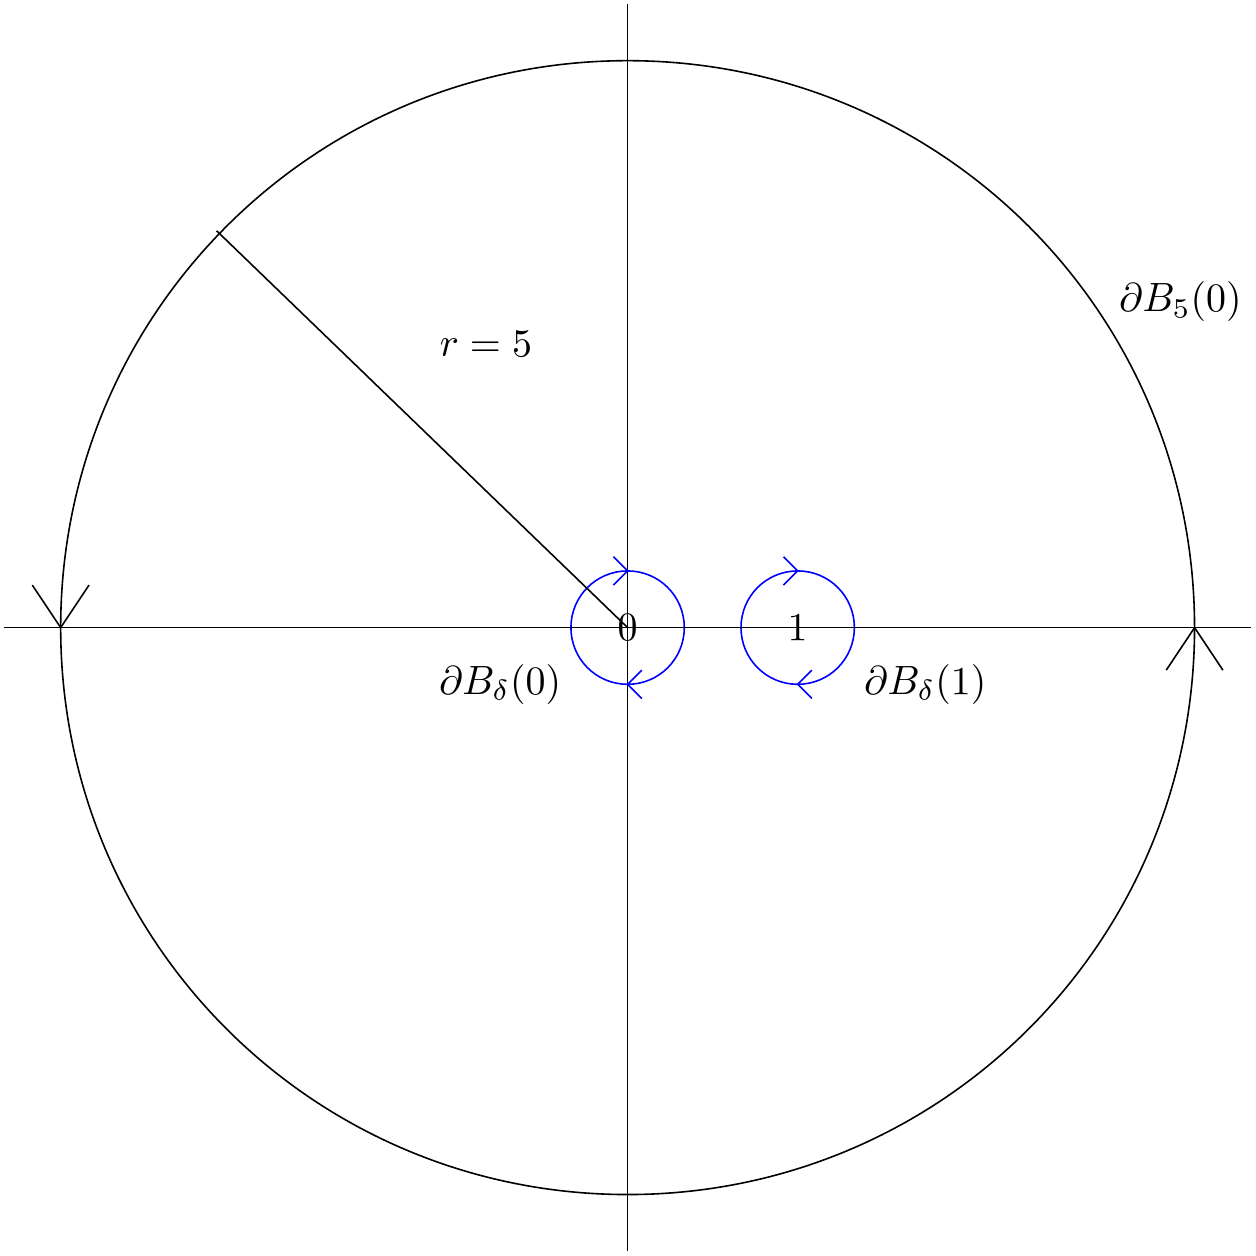
\includegraphics[scale=0.25]{Q6.png}
\end{center}

\begin{align*}
  25 \int_{\partial \partial B_5(0)} \frac{1}{z(z-1)} dz &= 25 \left[ \int_{\partial B_{\delta}(0)} \frac{1/(z-1)}{\left(z - 0\right)} dz + \int_{\partial B_{\delta}(1)} \frac{1/(z)}{\left(z - 1\right)} dz \right] \\
  &= 25 \left[ 2\pi i \cdot \left( \frac{1}{0-1} \right) + 2\pi i \cdot \left( \frac{1}{1} \right) \right] \\
  &= 50 \pi i \left( -1 + 1 \right) \\
  &= 0
\end{align*}

\vskip 0.5cm
\hrule 
\vskip 0.5cm



%%%%%%%%%%%%%%%%%%%%%%%%%%%%%%%%%%%%%%%%%%%%%%%%%%%%%%%%%%%%%%%%%
\begin{mathdefinitionbox}{Question 7}
\vskip 0.5cm
\begin{enumerate}[label=(\alph*)]
  \item Let $f : \R \rightarrow \R$ be the function defined as 
  \[ f(x) = \begin{cases}
    e^{-1/x^2}, \;\;x \neq 0 \\
    0, \;\;\;\;\;\;x = 0
  \end{cases} \]
  Show that $f$ is smooth (i.e. infinitely differentiable at $x = 0$), but that $f$ is not analytic in any neighborhood of $0$.

  \vskip 0.5cm
  \item Let $f : \C \rightarrow \C$ be the function defined as 
  \[ f(z) = \begin{cases}
    ^{-1/z^2}, \;\;z \neq 0 \\
    0, \;\;\;\;\;\;z = 0
  \end{cases} \]
  Show that $f$ is not even continuous at $z = 0$.
\end{enumerate}
\end{mathdefinitionbox}
%%%%%%%%%%%%%%%%%%%%%%%%%%%%%%%%%%%%%%%%%%%%%%%%%%%%%%%%%%%%%%%%%

\vskip 0.5cm
\underline{\textbf{Proof:}}

\begin{enumerate}[label=(\alph*)]
  \item Away from $x = 0$ the function is clearly smooth, so we just need to show smoothness at $x = 0$. First off, $f(x)$ is continuous at $x = 0$ since the left limit is clearly equal to zero and the right limit is 
  \[ \lim_{x \rightarrow 0+} e^{-\frac{1}{x^2}} = 0  \]
  whch agrees with the left limit.

  In fact, by standard applications of L'Hopital's Rule and Induction, we find that

  Let's show using induction that the $k$\emph{th} derivative is given by 
  \[ f^{(k)}(x) = p_{2k}(x) \frac{e^{-1/x^2}}{(x^2)^{2k}} \]
  for $x > 0$ and $x \leq 0$, where $p_{2k}(x)$ is a polynomial of degree at most $2k$.
  \vskip 0.5cm

  The $x \leq 0$ part clearly follows since the function itself is identically zero on that region.

  \vskip 0.5cm
  Now, for $x > 0$, the first derivative of $f(x)$ is 
  \[ f'(x) = \frac{-1}{2x^3} \cdot e^{-1/x^2} = \left(-\frac{1}{2}x\right) \frac{e^{-1/x^2}}{x^4} = \left(-\frac{1}{2}x\right) \frac{e^{-1/x^2}}{(x^2)^{2 \cdot 1}} \]
  which is exactly the form we need. This establishes the base case.

  \vskip 0.5cm
  Now suppose the claim holds for the $k$-th derivative. Then, 
  \begin{align*}
    f^{(k+1)}(x) &= p'_{2k}(x) \cdot \frac{e^{1/x^2}}{(x^2)^{2k}} + p_{2k}(x) \cdot \frac{ \frac{-1}{2x^3} e^{-1/x^2}}{x^2} + p_{2k}(x) \cdot e^{-1/x^2} \cdot \left(\frac{-4k}{x^{4k+1}}\right) \\
    &= \left[ x^2 \cdot p'_{2k}(x) - \frac{x}{2} \cdot p_{2k}(x) - 4k \cdot p_{2k}(x) \right] \frac{e^{-1/x^2}}{x^{4k+2}} \\
    &= \underbrace{\left[ x^2 \cdot p'_{2k}(x) - \frac{x}{2} \cdot p_{2k}(x) - 4k \cdot p_{2k}(x) \right]}_{deg = 2k+1} \frac{e^{-1/x^2}}{(x^2){2k+1}} \\
  \end{align*}

  This proves the claim. Further, we can prove by induction that $f^{(k)}(0) = 0$. For the base case, this is true because of the definition of the function. Now, assume it holds for the $k$-th case. To show that $f^{(k+1)}(0)$ exists at the origin, we need to show that $f^{(k)}$ has one sided limits which agree at $0$.

  \vskip 0.5cm 
  The left-limit of $f^{(k)}$ is just zero, from the definition of the function. The right hand limit is 

  \begin{align*}
    \lim_{x \rightarrow 0} \frac{ p_{2k}(x) \frac{e^{-1/x^2}}{(x^2)^{2k}} - 0}{x - 0} &= \lim_{x \rightarrow 0} p_{2k}(x) \frac{e^{-1/x^2}}{x^{2(k+1)}} \\
    &= p(0) \lim_{x \rightarrow 0} \frac{e^{-1/x^2}}{x^{2k+2}} \\
    &= 0
  \end{align*}
  where the last equality follows because we can prove 
  \[ \lim_{x \rightarrow 0} \frac{e^{-1/x^2}}{x^{2k+2}} = 0 \]
  for any $k$ using Induction and by repeatedly applying L'Hopital's rule.
  
  \vskip 0.5cm
  \emph{\textbf{Therefore, $f(x)$ is smooth.}}

  \vskip 0.5cm 
  But we very obviously have a problem! The taylor expansion for $f(x)$ is 
  \[ f(x) = \sum_{k = 0}^{\infty} \frac{f^{(k)}(0)}{k!} x^k \]
  and we've alredy shown that $f^{(k)}(0) = 0$ for all $k \in \mathbb{Z}_{\geq 0}$.

  whereas the values of $f(x)$ for any $x > 0$ are strictly non-zero. Thus, the function is not analytic in any neighborhood of $0$.

  \vskip 0.5cm
  \item Now consider the complex function 
  \[ f(z) = \begin{cases}
    e^{-1/z^2}, z \neq 0 \\
    0, z = 0
  \end{cases} \]

  This function is not even continuous, because if we take the limit $z = x + iy \rightarrow 0$ along the imaginary axis i.e. $x = 0$, we find 
  \begin{align*}
    \lim_{z \rightarrow 0} f(z) &= \lim_{x = 0, y \rightarrow 0} e^{-1/z^2}  \\
    &= \lim_{x = 0, y \rightarrow 0} e^{-1/(iy)^2} \\
    &= \lim_{y \rightarrow 0} e^{1/y^2} \\
  \end{align*}
  But this limit diverges!
\end{enumerate}



\vskip 0.5cm
\hrule 
\vskip 0.5cm



% %%%%%%%%%%%%%%%%%%%%%%%%%%%%%%%%%%%%%%%%%%%%%%%%%%%%%%%%%%%%%%%%%
% \begin{mathdefinitionbox}{Question }
% \vskip 0.5cm

% \end{mathdefinitionbox}
% %%%%%%%%%%%%%%%%%%%%%%%%%%%%%%%%%%%%%%%%%%%%%%%%%%%%%%%%%%%%%%%%%

% \vskip 0.5cm
% \underline{\textbf{Proof:}}

% \vskip 0.5cm
% \hrule 
% \vskip 0.5cm



\end{document}
